% easychair.tex,v 3.5 2017/03/15
\PassOptionsToPackage{x11names}{xcolor}

\documentclass{easychair}
%\documentclass[EPiC]{easychair}
%\documentclass[EPiCempty]{easychair}
%\documentclass[debug]{easychair}
%\documentclass[verbose]{easychair}
%\documentclass[notimes]{easychair}
%\documentclass[withtimes]{easychair}
%\documentclass[a4paper]{easychair}
%\documentclass[letterpaper]{easychair}

%------------------------------------------------------------------------------
%% DRAFT options
\usepackage{lineno}
\linenumbers

%% \usepackage{todonotes}
%% \setuptodonotes{inline}
%------------------------------------------------------------------------------

\usepackage{catchfilebetweentags}
\makeatletter

\newrobustcmd*\OrigExecuteMetaData[2][\jobname]{%
\CatchFileBetweenTags\CatchFBT@tok{#1}{#2}%
\global\expandafter\CatchFBT@tok\expandafter{%
\expandafter}\the\CatchFBT@tok
}%\OrigExecuteMetaData

\newrobustcmd*\ChkExecuteMetaData[2][\jobname]{%
\CatchFileBetweenTags\CatchFBT@tok{#1}{#2}%
\edef\mytokens{\detokenize\expandafter{\the\CatchFBT@tok}}
\ifx\mytokens\empty\PackageError{catchfilebetweentags}{the tag #2 is not found\MessageBreak in file #1 \MessageBreak called from \jobname.tex}{use a different tag}\fi%
}%\ChkExecuteMetaData

\renewrobustcmd*\ExecuteMetaData[2][\jobname]{%
\ChkExecuteMetaData[#1]{#2}%
\OrigExecuteMetaData[#1]{#2}%
}

\makeatother

\usepackage{idris2}

\usepackage{doc}
\usepackage{wrapfig}

% use this if you have a long article and want to create an index
% \usepackage{makeidx}

% In order to save space or manage large tables or figures in a
% landcape-like text, you can use the rotating and pdflscape
% packages. Uncomment the desired from the below.
%
% \usepackage{rotating}
% \usepackage{pdflscape}

\usepackage{amsfonts}


\usepackage{tikz}
\usetikzlibrary{automata, positioning, arrows}
\tikzset{
  ->, % makes the edges directed
  >=stealth', % makes the arrow heads bold
  node distance=2.5cm, % specifies the minimum distance between two nodes. Change if necessary.
  every state/.style={thick, fill=gray!10, minimum size=1cm}, % sets the properties for each ’state’ node
  initial text=$ $, % sets the text that appears on the start arrow
}

%% Front Matter
%%
% Regular title as in the article class.
%
\title{Type-safe Bidirectional Channels in Idris 2}

% Authors are joined by \and. Their affiliations are given by \inst, which indexes
% into the list defined using \institute
%
\author{Guillaume Allais\inst{1}}

% Institutes for affiliations are also joined by \and,
\institute{
  University of Strathclyde,
  Glasgow, Scotland, United Kingdom\\
  \email{guillaume.allais@strath.ac.uk}}

%  \authorrunning{} has to be set for the shorter version of the authors' names;
% otherwise a warning will be rendered in the running heads. When processed by
% EasyChair, this command is mandatory: a document without \authorrunning
% will be rejected by EasyChair

\authorrunning{Guillaume Allais}

% \titlerunning{} has to be set to either the main title or its shorter
% version for the running heads. When processed by
% EasyChair, this command is mandatory: a document without \titlerunning
% will be rejected by EasyChair
\titlerunning{Type-safe Bidirectional Channels in Idris 2}

\begin{document}

\maketitle

%------------------------------------------------------------------------------
\subsection*{Introduction}

Session types are a channel typing discipline ensuring that the
communication patterns of concurrent programs abide by a shared
protocol.
%
A meta-theoretical analysis of the typing discipline can then
ensure that the communicating processes will have good properties
e.g. deadlock-freedom.
%
We show how to use a linear dependently typed programming language
to define a direct and type-safe embedding of expressive binary
session types.

%------------------------------------------------------------------------------
\subsection*{Expressive Session Types}

\newcommand{\nat}{\ensuremath{\mathbb{N}}}
\newcommand{\recvar}[1]{\ensuremath{\mathit{#1}}}
\newcommand{\send}[2]{\ensuremath{!#1.~#2}}
\newcommand{\recv}[2]{\ensuremath{?#1.~#2}}
\newcommand{\select}[2]{\ensuremath{#1 \mathop{\oplus} #2}}
\newcommand{\offer}[2]{\ensuremath{#1 \mathop{\&} #2}}
\newcommand{\smallest}[2]{\ensuremath{\mu #1.~#2}}
\newcommand{\largest}[2]{\ensuremath{\nu #1.~#2}}
\newcommand{\stopsesh}{\ensuremath{\mathtt{end}}}

\noindent
\begin{wrapfigure}{r}{.5\textwidth}\centering%
  \vspace{-1cm}%
  \begin{align*}%
  p,~ q,~ \dots &
    \; ::= \; \recvar{x}
    \; | \; \smallest{x}{p}
    \; | \; \largest{x}{p} \\
    &
    \; | \; \send{A}{p}
    \; | \; \recv{A}{p}
    \; | \; \stopsesh{} \\
    &
    \; | \; \offer{p}{q}
    \; | \; \select{p}{q}
  \end{align*}

  \vspace{.5cm}

  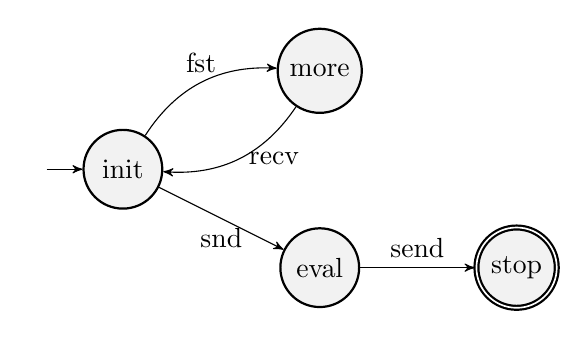
\begin{tikzpicture}
    \node[state, initial]                     (q1)  {init};
    \node[state, right of=q1, yshift=-1.25cm] (q2r) {eval};
    \node[state, above of=q2r]                (q2l) {more};
    \node[state, accepting, right of=q2r]     (q3)  {stop};
    \draw
      (q1) edge[bend left, above]  node{fst}       (q2l)
      (q1) edge[above, below]      node{snd}       (q2r)
      (q2l) edge[bend left, right] node{recv \nat} (q1)
      (q2r) edge[above]            node{send \nat} (q3);
  \end{tikzpicture}

  \vspace{1cm}

  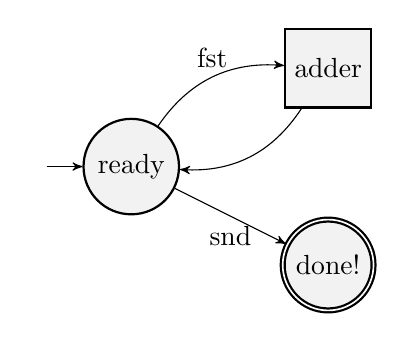
\begin{tikzpicture}
    \node[state, initial]                      (o1)  {ready};
    \node[state, right of=o1, , yshift=-1.25cm, accepting] (o2)  {done!};
    \node[state, shape=rectangle, above of=o2] (q1)  {adder};
    \draw
      (o1) edge[bend left, above] node{fst} (q1)
      (o1) edge[below]            node{snd} (o2)
      (q1) edge[bend left] (o1);
  \end{tikzpicture}
\end{wrapfigure}
%
Our session types are closed
under typed sends (\send{A}{\cdot}),
typed receives (\recv{A}{\cdot}),
branch offerings (\offer{\cdot}{\cdot}),
branch selections (\select{\cdot}{\cdot}),
and smallest (\smallest{x}{\cdot})
and largest (\largest{x}{\cdot}) fixpoints.

The session
$
\largest{x}{(\offer
  {(\recv{\nat}{\recvar{x}})}
  {(\send{\nat}{\stopsesh})})}
$
types a server for the ``adder'' protocol represented as
a finite state machine on the right hand side.
%
The server accepts an arbitrarily long sequence of natural numbers
(sent by a client repeatedly selecting the
\emph{more} = (\recv{\nat}{\recvar{x}}) branch)
before sending back their sum as a single number
(when the \emph{eval} = (\send{\nat}{\stopsesh}) branch is ultimately selected)
and terminating.
%
The encoding of the server's type uses a largest fixpoint
because the client is the one responsible
for ensuring the process terminates by eventually selecting
the \emph{eval} branch.

We can use nested fixpoint to describe more complex
protocols. For instance,
$
\largest{o}{(\offer{
  (\largest{x}{(\offer
    {(\recv{\nat}{\recvar{x}})}
    {(\send{\nat}{\recvar{o}})})}
  )}{\stopsesh})}
$
informally corresponds to the finite state machine
shown on the right hand side.
It types a server repeatedly offering to handle the adder
protocol described above (we replaced \stopsesh{} with
\recvar{o} to allow for the repetition) before stopping
when the client is done.


%------------------------------------------------------------------------------
\subsection*{Type-safe Implementation}

\paragraph{Pairs of Unityped Channels}
We represent a bidirectional channel
parametrised by a session type as a pair of unityped
unidirectional channels.
%
The key idea behind this safe implementation is to collect
all the types used in a protocol and to manufacture a big
sum type in which we can inject all of the values that need
to be exchanged.
%
The definition of this sum type is a type safe realisation of
Kiselyov and Sabry's open union type~\cite{DBLP:conf/haskell/KiselyovSS13}
using the encoding of scope-safe
De Bruijn indices~\cite{MANUAL:journals/math/debruijn72}
introduced by Brady in Idris 2's core~\cite{DBLP:conf/ecoop/Brady21}.
%
This gives us an encoding that has constant time injections and
(partial) projections in and out of the big sum type.

\paragraph{Dealing with Changing Sessions}
The session type, by design, changes after each communication
but the big sum type used when communicating across the
unityped channels needs to stay the same.
%
Our solution is to record an offset remembering where we currently
are in the protocol and thus allowing us to keep injecting values to
be sent into the initial shared sum type.
%
Our offsets are proven correct using a gadget that can be understood
as a cut down version of McBride's one hole
contexts~\cite{DBLP:conf/popl/McBride08}. Instead
of recording the full path followed by our programs in the finite
state machine describing the protocol,
we merely record a de-looped version.

\paragraph{Code Samples} We include code snippets showing the
types of \IdrisFunction{offer} and \IdrisFunction{select}
the dual primitives allowing branching.
%
Both are linear in their channel input; both involve a choice in the
form of a \IdrisType{Bool} value: \IdrisFunction{offer} gets it from
the other thread while \IdrisFunction{select} requires the caller to
pass it. In both cases, an appropriately stepped channel is return to
continue communicating.
%
\ExecuteMetaData[System/Concurrency/Session/RecursiveN.idr.tex]{offer}
\ExecuteMetaData[System/Concurrency/Session/RecursiveN.idr.tex]{select}

%------------------------------------------------------------------------------
\subsection*{Limitations and Future Work}

\paragraph{Encoding Uniqueness via Linear Types}
Unlike Brady's prior work in Idris 1~\cite{DBLP:journals/aghcs/Brady17},
we are using Idris 2 which does not currently have uniqueness types.
We are forced to use the linearity granted to us by
Quantitative Type Theory (QTT)~\cite{DBLP:conf/birthday/McBride16,DBLP:conf/lics/Atkey18}
to emulate uniquess via a library-wide invariant.
%
This adds a degree of noise and trust to the implementation.
We would ideally want a system combining both linearity and uniqueness
to benefit from enhanced expressivity and efficiency as described
by Marshall, Vollmer, and Orchard~\cite{DBLP:conf/esop/MarshallVO22}.

\paragraph{Small Runtime Overhead}
In the current version of our library, we compute a handful
of key offset values by induction over the protocol. Correspondingly
the protocol is not marked as erased anymore and, if compilation does
not specialise the relevant combinators agressively, then we may very
well be evaluating these relatively small computations at runtime.
%
As far as we understand, directly adding typed staging to Idris 2
through the use of a two-level type theory à la
Kov{\'{a}}cs~\cite{DBLP:journals/pacmpl/Kovacs22} would not be
enough to solve our issue: for typing purposes, the protocol does need
to persist through staging. But it should be possible to move it
from QTT's unrestricted to its erased modality.

\paragraph{Ergonomics}
We found writing the types of inner loops of programs with non-trivial
communication patterns to be tedious as they expose quite a lot of the
powerful but noisy encoding of syntaxes with binding we use.
Figuring out a more user-friendly surface syntax for our protocols is
left as future work.




%------------------------------------------------------------------------------
%% BIBLIOGRAPHY

\newpage
\bibliographystyle{plain}
%\bibliographystyle{alpha}
%\bibliographystyle{unsrt}
%\bibliographystyle{abbrv}
\bibliography{session}

\end{document}
